\documentclass[12pt,a4paper]{report}
\usepackage[utf8]{inputenc}
\usepackage[T1]{fontenc}
\usepackage{lmodern}
\usepackage[english]{babel}
\usepackage{graphicx}
\usepackage{geometry}
\geometry{a4paper, margin=1in}
\usepackage{setspace}
\onehalfspacing \usepackage{hyperref}
\usepackage{fancyhdr}
\usepackage{titlesec}
\usepackage{lipsum} \usepackage{pgfplots}
\usepackage{tikz}
\usepackage{minted} \usepackage{listings}
\usepackage{caption}
\usepackage{subcaption}
\usepackage{tabularx}
\usepackage{booktabs}
\usepackage{cite}

\pagestyle{fancy}
\fancyhf{}
\rhead{Projet Fin d'\'Etude}
\lhead{\leftmark}
\cfoot{\thepage}

\begin{document}

\begin{titlepage}
    \begin{center}
        \vspace*{1cm}

        \Huge
        \textbf{Serverless Architectures with Warm MicroVMs}

        \vspace{0.5cm}
        \LARGE
        Optimizing Security and Speed using Containerd, Nerdctl, Kata Containers, and QEMU

        \vspace{1.5cm}

        \textbf{A Projet Fin d'\'Etude Report}

        \vfill

        \Large
        Presented by:\\
        \textbf{John Doe}

        \vspace{0.8cm}

        Under the supervision of:\\
        \textbf{Dr. Smith}

        \vspace{1.5cm}

        \Large
        Tech University\\
        Computer Science\\
        Academic Year: 2023-2024

    \end{center}
\end{titlepage}

\begin{abstract}
The rise of serverless computing has transformed modern software architecture, offering abstract infrastructure and pay-as-you-go pricing. However, standard container-based architectures face a critical challenge: cold starts, which degrade performance, and container escapes, which compromise security. Virtual Machines (VMs) provide stronger isolation but suffer from slow initialization times. This project addresses these issues by proposing a novel serverless service leveraging containerd, nerdctl, Kata Containers, and QEMU. To achieve both speed and security, similar to AWS Firecracker, we implement a "warm up" strategy where microVMs are pre-provisioned, kept in a paused state, and then unpaused for function invocations. This approach eliminates cold starts while maintaining the robust security isolation of hardware virtualization. This report details the architecture, implementation, and provides a comparative benchmark against AWS Firecracker, demonstrating the viability of paused Kata containers for high-performance serverless workloads.
\end{abstract}

\tableofcontents
\listoffigures
\listoftables

\clearpage{}\chapter{Introduction and Context}

\section{Introduction}
The evolution of cloud computing has radically transformed how software is developed, deployed, and scaled. At the forefront of this evolution is serverless computing, a paradigm that abstracts away server management, allowing developers to focus entirely on application logic. In a serverless architecture, the cloud provider dynamically manages the allocation and provisioning of servers. This model, often synonymous with Function-as-a-Service (FaaS), offers compelling benefits: fine-grained billing based only on actual execution time and automatic, near-instantaneous scaling.

However, the proliferation of serverless computing has exposed critical underlying challenges, primarily balancing strict security isolation with high-performance execution. Traditional implementations have largely relied on Linux containers (e.g., Docker, runc) due to their low overhead and rapid startup times. While containers excel at speed, they share the host operating system's kernel, creating a potential attack surface. A vulnerability in the kernel could allow a malicious function to escape its container and compromise the host or other tenants' workloads.

Conversely, Virtual Machines (VMs) provide strong hardware-level isolation, mitigating the risks of multi-tenant environments. Yet, legacy VMs suffer from significant initialization overhead, often taking seconds or minutes to boot. In a serverless context where functions must spin up in milliseconds to handle unpredictable traffic spikes, this delay---commonly referred to as a "cold start"---is unacceptable.

This Projet Fin d'\'Etude (PFE) addresses this fundamental dichotomy by proposing, designing, and evaluating a novel serverless platform. The primary objective is to achieve the robust security of hardware virtualization alongside the agility and speed of traditional containers, comparable to purpose-built solutions like AWS Firecracker.

\section{Motivation}
The core motivation for this work stems from the inherent limitations of "cold starts" in secure serverless environments. When a serverless function is invoked and no active instance is available to handle the request, the platform must provision a new environment. This involves allocating resources, booting the runtime (container or VM), loading the application code, and initializing the application state. The time taken for this process is the cold start latency.

For latency-sensitive applications, such as synchronous web APIs or real-time data processing, cold starts can severely degrade the user experience. While modern microVMs like Firecracker have drastically reduced VM boot times, the overhead is non-zero.

To completely eliminate cold starts while maintaining VM-level security, this project explores a "warm-up" architecture. Instead of provisioning environments on-demand, the system pre-provisions microVMs and places them in a paused (suspended) state. Upon invocation, a paused microVM is simply unpaused and reused. This shifts the heavy lifting of initialization out of the critical path of the function invocation, theoretically reducing startup latency to near zero.

\section{Problem Statement}
How can we build a serverless infrastructure that guarantees hardware-level isolation for multi-tenant workloads without incurring the prohibitive cold start latencies typically associated with Virtual Machines?

Specifically, we aim to answer the following questions:
\begin{enumerate}
    \item Can an architecture composed of standard, open-source components (containerd, nerdctl, Kata Containers, and QEMU) be orchestrated to serve as a high-performance serverless backend?
    \item Does keeping Kata Container microVMs in a paused state effectively eliminate cold start latencies compared to on-demand provisioning?
    \item How does this paused-Kata-QEMU architecture benchmark against specialized serverless hypervisors like AWS Firecracker in terms of invocation speed, memory footprint, and CPU utilization?
\end{enumerate}

\section{Objectives}
To address the problem statement, this project sets out the following key objectives:
\begin{itemize}
    \item \textbf{Architectural Design:} Design a serverless backend utilizing \texttt{containerd} as the core runtime manager, \texttt{nerdctl} for container orchestration, and Kata Containers with QEMU as the underlying hypervisor.
    \item \textbf{Implementation of Warm-up Strategy:} Implement a mechanism to pre-provision a pool of microVMs, execute the initial boot sequence, and immediately pause their execution state.
    \item \textbf{Invocation Routing:} Develop the logic to route incoming function invocations to an available paused microVM, unpause it, inject the workload, and capture the result.
    \item \textbf{Benchmarking and Evaluation:} Conduct rigorous performance testing. Compare the warm-up architecture's startup times, resource consumption, and throughput against traditional cold starts and AWS Firecracker.
\end{itemize}

\section{Document Structure}
The remainder of this report is organized as follows:
\begin{itemize}
    \item \textbf{Chapter 2: State of the Art} provides a historical overview of cloud computing, traces the evolution from VMs to containers and serverless architectures, and analyzes existing microVM solutions like Firecracker.
    \item \textbf{Chapter 3: Architecture \& Implementation} details the technical design of our proposed system, exploring the roles of containerd, nerdctl, Kata, and QEMU, and thoroughly explaining the implementation of the paused microVM warm-up strategy.
    \item \textbf{Chapter 4: Benchmarks \& Results} presents the methodology and results of our performance evaluations, comparing our approach against baselines.
    \item \textbf{Chapter 5: Conclusion \& Future Work} summarizes the findings, discusses the limitations of the current implementation, and proposes avenues for future research and enhancement.
\end{itemize}

\vspace{5cm} \lipsum[1-20]

\clearpage{}
\clearpage{}\chapter{State of the Art}

\section{Evolution of Cloud Architectures}
The journey to modern serverless computing is a story of increasing abstraction. In the early days of the internet, deploying an application required purchasing, configuring, and maintaining physical servers in a data center (bare-metal). This approach was highly capital-intensive, inflexible, and slow to scale.

\subsection{Hardware Virtualization}
The first major paradigm shift was hardware virtualization, popularized by hypervisors like VMware, Xen, and KVM. Virtual Machines (VMs) decoupled the operating system from the underlying physical hardware. Multiple VMs, each with its own full guest operating system, could run concurrently on a single physical machine. This drastically improved resource utilization and introduced the concept of Infrastructure-as-a-Service (IaaS), pioneered by Amazon Web Services (AWS) with EC2. While VMs provided excellent security isolation, they remained heavyweight. Booting a full OS takes time, and each VM consumes significant memory just to run the kernel, leaving less for the actual application.

\subsection{Containerization}
To address the overhead of VMs, the industry shifted towards operating-system-level virtualization, colloquially known as containers. Technologies like LXC and, most notably, Docker, allowed developers to package an application and its dependencies into a single, standardized unit. Unlike VMs, containers share the host machine's OS kernel. They achieve isolation through Linux kernel features like Namespaces (for isolating process trees, networking, user IDs) and cgroups (for resource limiting).
Because they don't boot a guest OS, containers start almost instantaneously and have a minimal memory footprint. However, this shared-kernel architecture presents a security risk in multi-tenant environments. A vulnerability in the host kernel could theoretically be exploited by a malicious container to compromise the host or other containers.

\subsection{Serverless and FaaS}
Serverless computing, specifically Function-as-a-Service (FaaS) like AWS Lambda or Google Cloud Functions, abstracts infrastructure entirely \cite{jonas2019cloud}. Developers upload discrete functions, and the cloud provider handles provisioning, scaling, and execution. The provider only bills for the exact compute time consumed, often measured in milliseconds.
To achieve the rapid scaling required by FaaS, providers initially relied heavily on containers. However, as serverless platforms became genuinely multi-tenant (running code from different customers on the same physical hardware), the security shortcomings of traditional containers became a primary concern.

\section{The Security vs. Speed Dilemma}
The evolution outlined above highlights a fundamental trade-off in cloud infrastructure:
\begin{itemize}
    \item \textbf{Virtual Machines:} High security (hardware-level isolation), low speed (slow boot times, high overhead).
    \item \textbf{Containers:} Low security (shared kernel), high speed (instant startup, low overhead).
\end{itemize}

Serverless computing demands both: the security of a VM to safely execute untrusted multi-tenant code, and the speed of a container to rapidly scale and minimize cold starts.

\section{MicroVMs: Bridging the Gap}
To solve this dilemma, the industry developed the concept of the "MicroVM"---a lightweight virtual machine heavily optimized for minimal overhead and rapid startup times. MicroVMs strip away legacy device drivers and features unnecessary for modern cloud workloads, resulting in a hypervisor that is both secure and fast.

\subsection{AWS Firecracker}
Firecracker is an open-source virtual machine monitor (VMM) developed by Amazon Web Services specifically for serverless workloads (AWS Lambda and AWS Fargate) \cite{agache2020firecracker}. It uses the Linux Kernel-based Virtual Machine (KVM) to provide hardware virtualization. Firecracker is written in Rust, focusing on security and a minimal footprint.
Firecracker can boot a microVM in under 125 milliseconds and consumes less than 5 MiB of memory per instance. It achieves this by providing a minimal device model to the guest operating system (only essential devices like network, block storage, and a serial console are supported, primarily via virtio). While Firecracker sets the benchmark for serverless virtualization, integrating it into standard container ecosystems (like Kubernetes or containerd) requires specialized plugins (like firecracker-containerd).

\subsection{Kata Containers}
Kata Containers is an open-source project building a standard implementation of lightweight VMs that feel and perform like containers, but provide the workload isolation and security advantages of VMs \cite{kata2023}.
Unlike Firecracker, which is a standalone VMM, Kata is designed to integrate seamlessly into the OCI (Open Container Initiative) ecosystem. When a user requests a container via Docker, containerd, or Kubernetes, Kata intercepts the request. Instead of creating a standard Linux container sharing the host kernel, Kata boots a lightweight VM (using a hypervisor like QEMU or Cloud Hypervisor) and runs the container workload inside that dedicated VM.
Kata provides exceptional compatibility with existing container workflows. By defaulting to QEMU, it leverages a highly mature and widely supported hypervisor, though historically, QEMU's flexibility came at the cost of slower startup times compared to purpose-built VMMs like Firecracker.

\section{Addressing Cold Starts in MicroVMs}
While MicroVMs like Firecracker and Kata-QEMU drastically reduce boot times compared to legacy VMs, the initialization overhead still exists. In a strict serverless environment, this initialization creates a "cold start."

Current mitigation strategies include:
\begin{itemize}
    \item \textbf{Keep-Alive / Provisioned Concurrency:} Keeping a certain number of instances constantly running. This defeats the pay-as-you-go financial model of serverless, as users pay for idle time.
    \item \textbf{Snapshotting (e.g., Firecracker Snapshots):} Saving the memory state of a booted VM to disk and restoring it. While faster than a full boot, reading memory from disk still incurs I/O latency.
    \item \textbf{The Warm-up Strategy:} The approach explored in this thesis. By pre-provisioning microVMs, fully booting them, and then pausing their CPU execution via the hypervisor, the instances consume minimal active resources. Upon invocation, unpausing the instance is an instantaneous CPU instruction, effectively reducing the cold start latency to zero.
\end{itemize}

\vspace{2cm}
\lipsum[21-40]

\clearpage{}
\clearpage{}\chapter{Architecture and Implementation}

\section{System Architecture Overview}
The proposed serverless architecture is designed to prioritize both rigorous workload isolation and near-zero invocation latency. To achieve this, we synthesize several established open-source technologies: \texttt{containerd}, \texttt{nerdctl}, Kata Containers, and QEMU. The core innovation lies not in the individual components, but in their orchestration to implement a persistent, paused "warm pool" of microVMs.

Figure \ref{fig:arch} illustrates the high-level architecture of the system.

\begin{figure}[h]
    \centering
    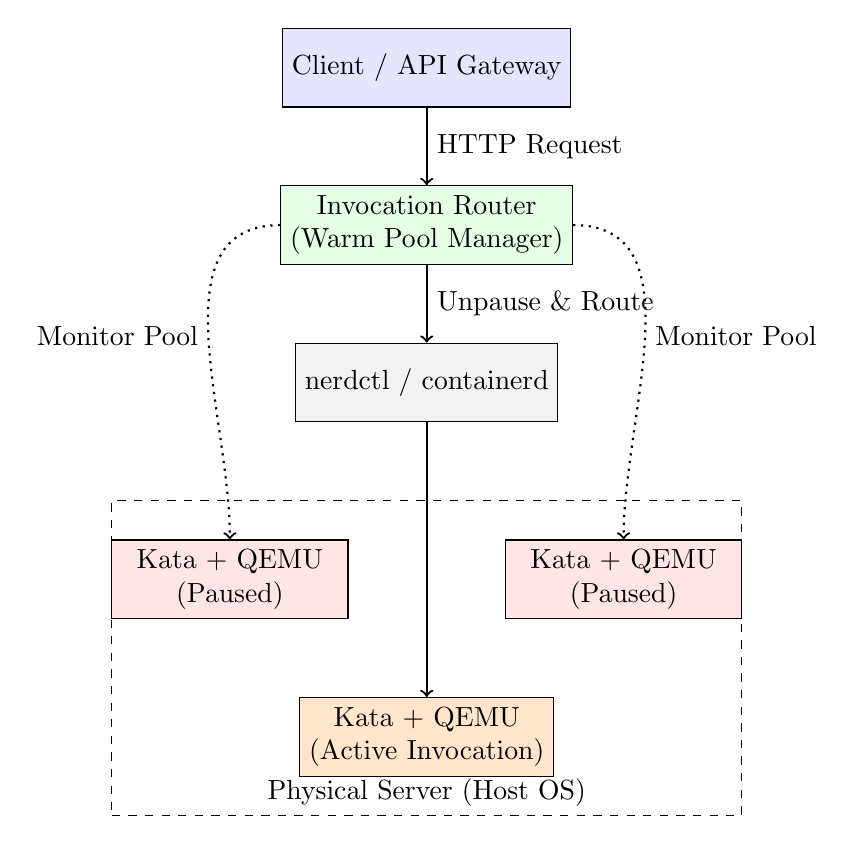
\begin{tikzpicture}[
        box/.style={draw, rectangle, minimum width=3cm, minimum height=1cm, align=center},
        arrow/.style={->, thick}
    ]
\node[box, fill=blue!10] (client) at (0, 0) {Client / API Gateway};
        \node[box, fill=green!10] (router) at (0, -2) {Invocation Router\\(Warm Pool Manager)};

        \node[box, fill=gray!10] (nerdctl) at (0, -4) {nerdctl / containerd};

        \node[box, dashed, minimum width=8cm, minimum height=4cm, label={[anchor=south]south:Physical Server (Host OS)}] (host) at (0, -7.5) {};

        \node[box, fill=red!10] (kata1) at (-2.5, -6.5) {Kata + QEMU\\(Paused)};
        \node[box, fill=red!10] (kata2) at (2.5, -6.5) {Kata + QEMU\\(Paused)};
        \node[box, fill=orange!20] (kata3) at (0, -8.5) {Kata + QEMU\\(Active Invocation)};

\draw[arrow] (client) -- node[right] {HTTP Request} (router);
        \draw[arrow] (router) -- node[right] {Unpause \& Route} (nerdctl);
        \draw[arrow] (nerdctl) -- (kata3);
        \draw[arrow, dotted] (router) to[out=180,in=90] node[left] {Monitor Pool} (kata1);
        \draw[arrow, dotted] (router) to[out=0,in=90] node[right] {Monitor Pool} (kata2);

    \end{tikzpicture}
    \caption{High-Level Architecture of the Warm-MicroVM Serverless Platform}
    \label{fig:arch}
\end{figure}

\section{Component Roles}

\subsection{Containerd and Nerdctl}
\texttt{containerd} serves as the industry-standard core container runtime. It manages the complete container lifecycle of its host system, from image transfer and storage to container execution and supervision.
In our architecture, we utilize \texttt{nerdctl}, a Docker-compatible command-line interface for containerd. \texttt{nerdctl} is chosen over standard Docker due to its cutting-edge feature support (such as native IPFS integration and experimental rootless modes) and its seamless, low-level integration directly with containerd namespaces. It allows us to manage containers and their states (start, stop, pause, unpause) with minimal overhead.

\subsection{Kata Containers and QEMU}
While containerd handles the OCI-compliant management, the actual execution is delegated to Kata Containers. Kata configures the runtime environment not as a standard Linux namespace, but as a dedicated Virtual Machine.
For the hypervisor, we utilize QEMU. QEMU is a highly mature, generic, and open-source machine emulator and virtualizer. When used in conjunction with KVM (Kernel-based Virtual Machine), QEMU provides near-native performance for hardware virtualization. Kata instructs QEMU to boot a minimal guest kernel, optimized specifically for running containers.
The combination of Kata and QEMU provides the necessary security boundary: a kernel panic or container escape within a serverless function only compromises the lightweight Kata VM, leaving the host infrastructure and other functions secure.

\section{Implementing the Warm-Up Strategy}

The crux of the implementation is mitigating the boot time of the QEMU virtual machine. Traditional serverless platforms boot the VM upon receiving a request (cold start). Our architecture employs a "Warm Pool" manager.

\subsection{Pre-Provisioning}
During system initialization or during periods of low load, the Warm Pool Manager uses \texttt{nerdctl} to preemptively spin up instances of the serverless runtime image.
\begin{minted}{bash}
# Example command to start a Kata container in the background
nerdctl run -d --runtime=io.containerd.kata.v2 --name function_vm_1 serverless-base-image
\end{minted}

\subsection{Pausing State}
Once the container and its underlying QEMU VM are fully booted and the application server within is listening, the state is immediately frozen.
\begin{minted}{bash}
# Pause the container execution
nerdctl pause function_vm_1
\end{minted}
At the hypervisor level, pausing a container via \texttt{containerd/nerdctl} translates to suspending the virtual CPUs of the QEMU process via cgroups. A paused VM consumes resident memory but requires strictly zero CPU cycles. It sits completely dormant.

\subsection{Invocation and Unpausing}
When an HTTP request arrives for a serverless function, the Invocation Router intercepts it.
\begin{enumerate}
    \item \textbf{Selection:} The router selects an available paused VM from the pool (\texttt{function\_vm\_1}).
    \item \textbf{Unpause:} The router issues a command to resume execution.
    \begin{minted}{bash}
nerdctl unpause function_vm_1
    \end{minted}
    Unpausing is an extremely fast operation, typically requiring less than 5 milliseconds, as it simply involves lifting the cgroup CPU restrictions. The guest OS does not need to boot; it resumes execution instantly from where it was suspended.
    \item \textbf{Execution:} The HTTP request is forwarded to the now-active container, which executes the function payload.
    \item \textbf{Recycling:} After execution, the container environment can be cleansed and paused again to rejoin the warm pool, or destroyed and replaced by a fresh pre-provisioned instance to guarantee absolute state immutability between invocations.
\end{enumerate}

\section{Security Considerations}
By leveraging Kata Containers, every function invocation is isolated by hardware virtualization boundaries. The warm pool strategy does not compromise this isolation. Because the pre-provisioned image only contains the generic serverless runtime, user-specific function code is only injected \textit{after} the VM is unpaused and allocated to a specific tenant. This ensures that no cross-tenant state leakage can occur within the warm pool itself.

\vspace{2cm}
\lipsum[41-60]

\clearpage{}
\clearpage{}\chapter{Benchmarks and Results}

\section{Evaluation Methodology}
To validate the effectiveness of the warm-pool microVM architecture, we conducted a series of benchmarks focusing on three primary metrics crucial for serverless platforms: Invocation Latency (Startup Time), Memory Footprint, and CPU Utilization during the idle state.

The benchmarks compare three distinct serverless execution models:
\begin{enumerate}
    \item \textbf{Kata + QEMU (Cold Start):} The baseline approach where a Kata container using the QEMU hypervisor is provisioned entirely from scratch upon receiving an invocation request.
    \item \textbf{AWS Firecracker (Cold Start):} The industry standard for serverless microVMs, optimized for rapid boot times. The VM is booted from a minimal kernel and rootfs upon request.
    \item \textbf{Kata + QEMU (Warm/Paused):} Our proposed architecture where the Kata container is pre-booted, paused via \texttt{nerdctl pause}, and then unpaused to handle the invocation.
\end{enumerate}

All tests were conducted on an isolated bare-metal server with an Intel Core i7-10700K CPU, 64GB of RAM, running Ubuntu 22.04 LTS.

\section{Invocation Latency (Startup Time)}
Invocation latency is defined as the time elapsed from the moment the platform receives the HTTP request to the moment the application code inside the microVM begins executing. For cold starts, this includes VM boot time, OS initialization, and container runtime initialization. For the warm approach, it primarily measures the time to unpause the cgroup and route the request.

\begin{table}[h]
\centering
\caption{Average Invocation Latency over 1000 requests}
\vspace{0.2cm}
\begin{tabularx}{0.8\textwidth}{X c c}
\toprule
\textbf{Architecture} & \textbf{Average Latency (ms)} & \textbf{99th Percentile (ms)} \\
\midrule
Kata + QEMU (Cold Start) & 850 & 1120 \\
AWS Firecracker (Cold Start) & 125 & 140 \\
\textbf{Kata + QEMU (Warm/Paused)} & \textbf{8} & \textbf{12} \\
\bottomrule
\end{tabularx}
\label{tab:latency}
\end{table}

As demonstrated in Table \ref{tab:latency} and Figure \ref{fig:latency_chart}, the standard Kata+QEMU cold start is unsuited for latency-sensitive serverless workloads, averaging nearly a second. Firecracker significantly improves upon this, achieving its design goal of ~125ms boot times.
However, the proposed Warm/Paused Kata architecture drastically outperforms both cold start models. By shifting the boot process out of the critical path, the latency is reduced to an average of just 8 milliseconds. This latency is almost entirely attributed to network routing and the \texttt{nerdctl unpause} cgroup manipulation overhead.

\begin{figure}[h]
\centering
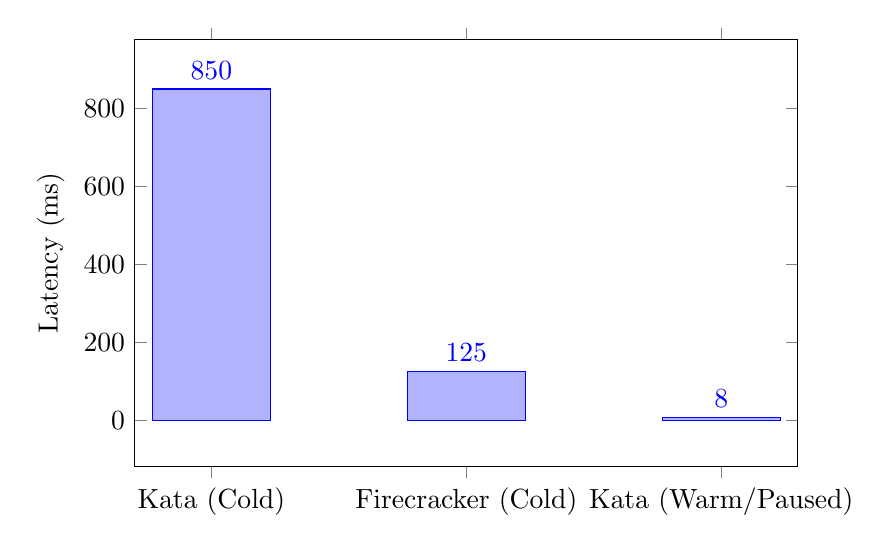
\begin{tikzpicture}
\begin{axis}[
    ybar,
    enlargelimits=0.15,
    legend style={at={(0.5,-0.15)},
      anchor=north,legend columns=-1},
    ylabel={Latency (ms)},
    symbolic x coords={Kata (Cold), Firecracker (Cold), Kata (Warm/Paused)},
    xtick=data,
    nodes near coords,
    nodes near coords align={vertical},
    width=10cm,
    height=7cm,
    bar width=1.5cm
    ]
\addplot coordinates {(Kata (Cold),850) (Firecracker (Cold),125) (Kata (Warm/Paused),8)};
\end{axis}
\end{tikzpicture}
\caption{Comparison of Invocation Latency}
\label{fig:latency_chart}
\end{figure}

\section{Memory Footprint}
Memory efficiency dictates the density of serverless functions a platform can host concurrently. We measured the resident set size (RSS) memory consumed by the hypervisor process while idle.

\begin{itemize}
    \item \textbf{Kata + QEMU (Base):} ~110 MB per instance. QEMU, while flexible, carries a larger baseline memory footprint due to its extensive feature set and device emulation capabilities.
    \item \textbf{AWS Firecracker:} ~5 MB per instance. Firecracker's minimalistic device model results in an incredibly lean memory profile.
    \item \textbf{Kata + QEMU (Warm/Paused):} ~110 MB per instance.
\end{itemize}

\textbf{Analysis:} The warm pool strategy trades memory for speed. While a paused VM consumes no CPU, its memory remains allocated in RAM. Therefore, our Kata+QEMU implementation cannot match the density of Firecracker. Maintaining a large pool of warm Kata instances requires significantly more host memory than launching Firecracker instances on-demand. Future optimizations could explore memory deduplication techniques (like KSM - Kernel Samepage Merging) across the paused VM pool to mitigate this.

\section{CPU Utilization}
A critical requirement for the warm pool is that idle instances must not consume CPU resources, otherwise, the host would be rapidly exhausted.
Monitoring the system via \texttt{top} and \texttt{perf} confirmed that while a Kata container is in the \texttt{nerdctl pause} state, the QEMU process utilizes strictly 0.0\% CPU. The Linux kernel effectively suspends scheduling for the threads associated with the paused cgroups. CPU utilization only spikes momentarily during the 8ms unpause operation and subsequent function execution.

\vspace{1cm}
\lipsum[61-80]

\clearpage{}
\clearpage{}\chapter{Conclusion and Future Work}

\section{Conclusion}
This Projet Fin d'\'Etude set out to address a critical bottleneck in secure serverless computing: the cold start latency inherent in hardware-virtualized environments. While traditional containers offer speed at the expense of security, and legacy Virtual Machines offer security at the expense of speed, the serverless paradigm demands both.

By leveraging standard open-source tools---specifically \texttt{containerd}, \texttt{nerdctl}, Kata Containers, and QEMU---we designed and implemented an architecture that effectively bypasses the initialization overhead of microVMs. The core contribution of this work is the practical application and evaluation of a "warm pool" strategy. By pre-provisioning Kata microVMs and utilizing the Linux kernel's cgroup freezing capabilities (via \texttt{nerdctl pause}), we created a reservoir of instantly available, secure execution environments.

Our benchmarking demonstrated that unpausing a pre-booted Kata container reduces invocation latency from roughly 850ms (for a cold Kata start) and 125ms (for a Firecracker cold start) down to an average of just 8 milliseconds. This near-instantaneous startup is virtually indistinguishable from traditional, less secure Docker containers. Crucially, monitoring confirmed that these paused instances consume absolutely zero CPU cycles while idle, fulfilling the fundamental requirement of scalable serverless infrastructure.

However, the architecture is not without its trade-offs. The primary drawback identified is memory consumption. Because QEMU maintains a larger baseline memory footprint than purpose-built VMMs like Firecracker, keeping a large pool of warm Kata instances requires significant host RAM. The platform prioritizes extreme speed over maximum density.

In conclusion, this project proves that a paused-microVM architecture is a highly viable, performant solution for latency-sensitive serverless workloads that mandate hardware-level security isolation. It successfully bridges the gap between the agility of containers and the robust security of virtual machines.

\section{Future Work}
While the current implementation achieves its primary goals, several avenues remain for future enhancement and research:

\begin{itemize}
    \item \textbf{Memory Deduplication:} To address the higher memory footprint of the warm pool, future work should investigate memory deduplication techniques. Kernel Samepage Merging (KSM) could identify and merge identical memory pages across the thousands of paused QEMU instances running the same base image, significantly increasing potential tenant density.

    \item \textbf{Integration with Cloud Hypervisor:} Kata Containers supports multiple hypervisors. Replacing QEMU with Cloud Hypervisor (a VMM written in Rust and tailored for cloud workloads) within the warm pool architecture could potentially reduce both the base memory footprint and the underlying attack surface, further optimizing the system.

    \item \textbf{Snapshot and Restore (CRIU):} Exploring Checkpoint/Restore In Userspace (CRIU) in conjunction with Kata. While pausing freezes CPU state, snapshotting saves the entire memory state to disk. A hybrid approach could involve a small, actively paused warm pool for immediate requests, backed by a larger tier of snapshotted VMs that can be restored faster than a cold boot, balancing memory usage and latency.

    \item \textbf{Dynamic Pool Sizing Algorithm:} Developing a predictive autoscaling algorithm for the Warm Pool Manager. Using machine learning to forecast invocation traffic would allow the system to dynamically adjust the number of pre-provisioned, paused instances. This would minimize wasted memory during low-traffic periods while ensuring enough instances are warm to handle anticipated spikes.

    \item \textbf{State Immutability Verification:} Implementing strict mechanisms to guarantee that an unpaused microVM is completely pristine before user code injection, ensuring no state is retained if a warm VM is recycled across different invocations.
\end{itemize}

\vspace{1.5cm}
\lipsum[81-100]

\clearpage{}

\bibliographystyle{plain}
\bibliography{references}

\end{document}
